\chapter{Implementasi dan Pengujian}
\label{chap:implementasi}

Pada bab ini terdapat tiga bagian, yaitu Implementasi Perangkat Lunak, Pengujian Perangkat Lunak dan contoh simulasi. Bagian implementasi akan menjelaskan tentang lingkungan pengembangan perangkat lunak dan hasil implementasi. Bagian pengujian akan berisi hasil pengujian fungsional terhadap perangkat lunak yang telah dibangun dan bagian terakhir yaitu contoh simulasi.

\section{Implementasi}
\label{sec:implementasi}

\subsection{Implementasi}
Implementasi dilakukan dengan menggunakan laptop dengan spesifikasi sebagai berikut :
\begin{enumerate}
	\item \textit{Processor} : Intel(R) Core(TM) i5-4200U CPU @ 1.60GHz 2.30GHz
	\item RAM : 4.00 GB
	\item Sistem Operasi : Windows 10 Pro 64-bit
	\item Versi Netbeans : 8.0.2
	\item Microsoft Excel : 2013
\end{enumerate}

\subsection{Hasil Implementasi}
\begin{enumerate}
	\item Tampilan Bobot Ketetanggaan
	
	
	Seperti yang telah dijelaskan pada bab \ref{chap:perancangan}, tampilan ini berfungsi untuk mengisi atribut dari masing-masing wirausaha. \textit{User} dapat memilih atribut mana yang akan dijadikan sebagai ketetanggaan dari masing-masing wirausaha dengan cara men-\textit{checklist checkbox} atribut yang diinginkan. (Gambar \ref{fig:tampilanBobot1})
	
	
	\begin{figure} [H]
	\centering  
	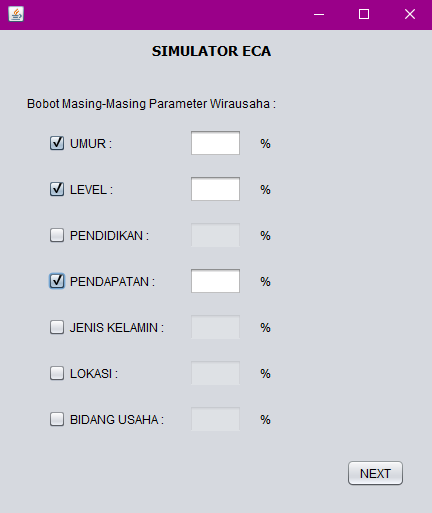
\includegraphics[width=8cm, height=10cm]{tampilanImplementasiBobot} 
		\caption[Gambar Tampilan Bobot Ketetanggaan]{Gambar Tampilan Bobot Ketetanggaan pada saat men-\textit{checklist checkbox}}
	\label{fig:tampilanBobot1} 
\end{figure}

	\begin{figure} [H]
	\centering  
	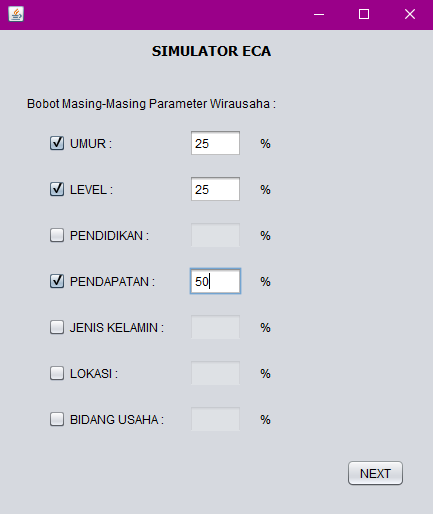
\includegraphics[width=8cm, height=10cm]{tampilanImplementasiBobot1} 
		\caption[Gambar Tampilan Bobot Ketetanggaan]{Gambar Tampilan Bobot Ketetanggaan pada saat mengisi bobot masing-masing atribut}
	\label{fig:tampilanBobot2} 
\end{figure}
	
	Pada implementasi ini, sebagai contoh \textit{user} memilih 3 atribut yaitu umur, level dan pendapatan. Masing-masing bobotnya yaitu 25\%, 25\% dan 50\%. 

	\item Tampilan Kondisi Ketetanggaan
	
	Pada tampilan ini, \textit{user} diminta untuk mengisi relasi ketetanggaan pada atribut yang telah dipilih sebelumnya. (Gambar \ref{fig:tampilantetangga})
	
	\begin{figure} [H]
	\centering  
	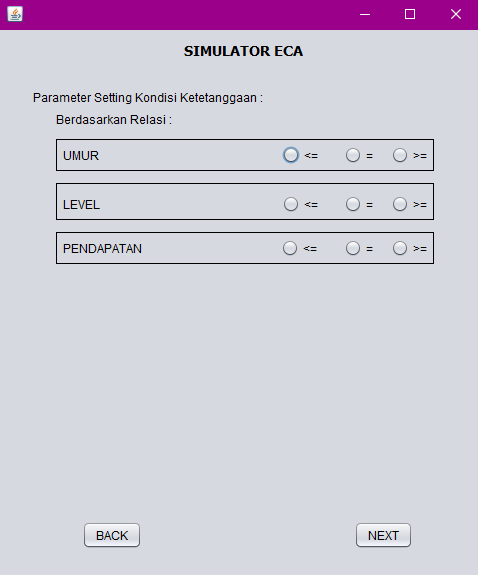
\includegraphics[width=8cm, height=10cm]{tampilanImplementasiKetetanggaan} 
		\caption[Gambar Tampilan Kondisi Ketetanggaan]{Gambar Tampilan Kondisi Ketetanggaan untuk atribut yang telah dipilih sebelumnya.}
	\label{fig:tampilantetangga} 
\end{figure}

	%\textit{User} dapat mengisi relasi melalui \textit{radio button} dan \textit{user} hanya bisa memilih salah satu diantara tiga relasi tersebut. (Gambar \ref{fig:tampilantetangga1})
	
	\begin{figure} [H]
	\centering  
	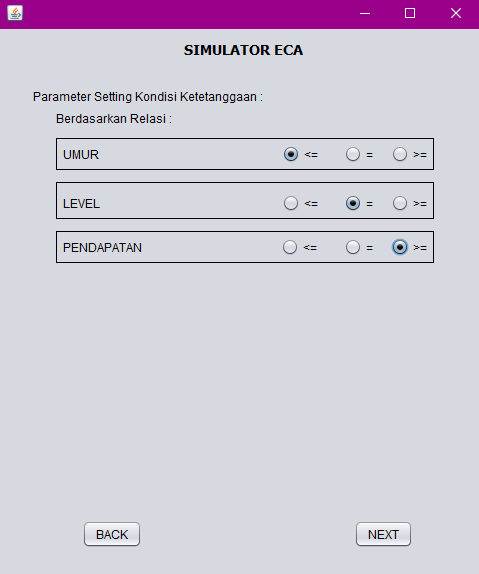
\includegraphics[width=8cm, height=10cm]{tampilanImplementasiKetetanggaan1} 
		\caption[Gambar Tampilan Kondisi Ketetanggaan]{Gambar Tampilan Kondisi Ketetanggaan pada saat mengisi relasi ketetanggaan}
	\label{fig:tampilantetangga1} 
\end{figure}
	Pada implementasi ini, \textit{user} mengisi masing-masing relasi ketetanggaan untuk umur yaitu kurang dari sama dengan, level wirausaha relasinya sama dengan dan pendapatan relasinya lebih dari sama dengan.

	\item Tampilan Kondisi Eksternal
	
	Pada tampilan ini, \textit{user} akan mengisi bobot masing-masing faktor publik. Jumlah dari seluruh bobot harus 100\%. \textit{User} mengisi masing-masing bobot dengan 5\%, 5\%, 10\%, 10\%, 10\%, 5\%, 10\%, 5\%, 10\%, 10\%, 10\% dan 10\%. Bobot-bobot ini nantinya akan dikalikan dengan nilai dari masing-masing faktor publik yang dapat dilihat pada tabel \ref{dataPublik}. (Gambar \ref{fig:tampilaneksternal1})
	
		\begin{figure} [H]
	\centering  
	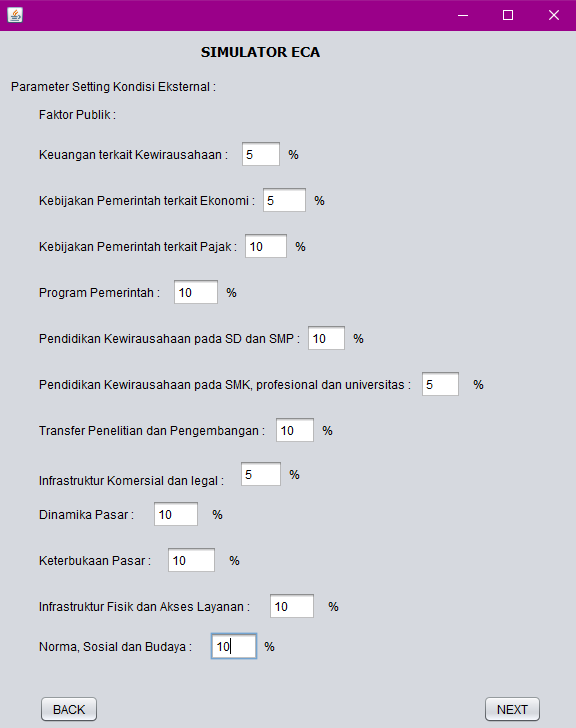
\includegraphics[width=9cm, height=11cm]{tampilanImplementasiEksternal} 
		\caption[Gambar Tampilan Ketetanggaan]{Gambar Tampilan Kondisi Eksternal pada saat mengisi bobot faktor publik}
	\label{fig:tampilaneksternal1} 
\end{figure}

	\item Tampilan Data Wirausaha
	
 	Pada tampilan data wirausaha \textit{user} dapat meng-klik \textit{button} "OPEN FILE" yang fungsinya untuk membuka \textit{file} data wirausaha yang akan disimulasikan. Data wirausaha berisi jenis kelamin, umur, usia bisnis, kategori usaha, subkategori usaha, pendidikan, lokasi, pendapatan, level dan point \ref{fig:formatFile}. Point merupakan hasil perhitungan masing-masing wirausaha pada kondisi internal. (Gambar \ref{fig:tampilandata})
	
		\begin{figure} [H]
	\centering  
	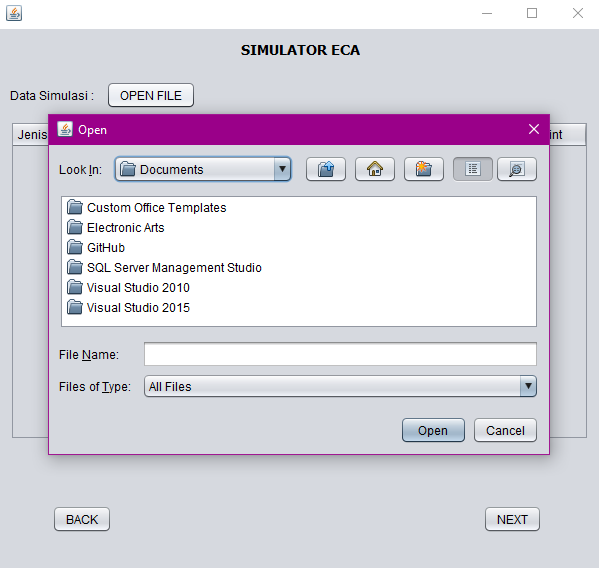
\includegraphics[width=10cm, height=10cm]{tampilanImplementasiData} 
		\caption[Gambar Tampilan Data Wirausaha]{Gambar Tampilan Data Wirausaha pada saat membuka \textit{button} "OPEN FILE"}
	\label{fig:tampilandata} 
\end{figure}

Berikut merupakan tampilan data wirausaha (data \textit{dummy}) yang telah dipilih oleh \textit{user}. (Gambar \ref{fig:tampilandata1})
	
		\begin{figure} [H]
	\centering  
	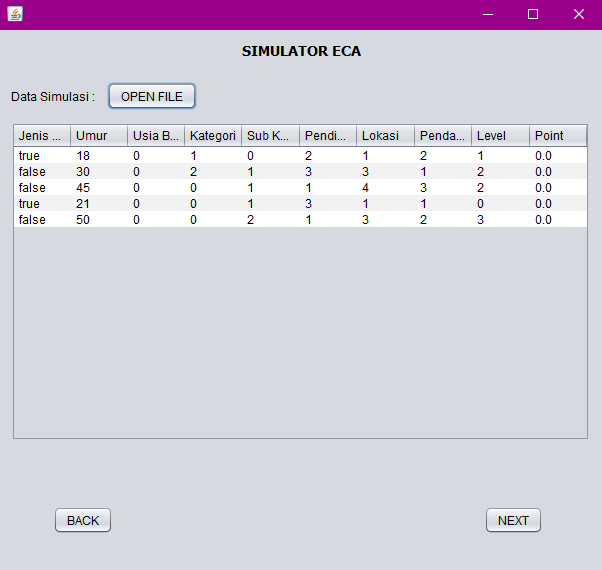
\includegraphics[width=10cm, height=10cm]{tampilanImplementasiData1} 
		\caption[Gambar Tampilan Data Wirausaha]{Gambar Tampilan Data Wirausaha saat menampilkan isi dari file}
	\label{fig:tampilandata1} 
\end{figure}

	\item Tampilan Simulasi
	
	Pada tampilan ini \textit{user} diminta untuk mengisi bobot dari a,b,c,threshold dan periode yang digunakan untuk menjalankan simulasi. Total nilai dari a,b dan c harus 1. Setelah mengisi masing-masing nilai, \textit{user} dapat melakukan simulasi dengan cara meng-klik \textit{button} "SIMULATE". (Gambar \ref{fig:tampilansimulasi})
	
		\begin{figure} [H]
	\centering  
	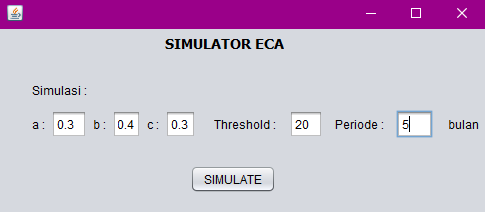
\includegraphics[width=8cm, height=4cm]{tampilanImplementasiSimulasi1} 
		\caption[Gambar Tampilan Simulasi]{Gambar Tampilan Simulasi pada saat mengisi bobot a,b,c,threshold dan periode}
	\label{fig:tampilansimulasi} 
\end{figure}

\textit{User} mengisi nilai a,b,c masing-masingnya yaitu 0.3, 0.4 dan 0.3, sedangkan \textit{threshold} atau nilai ambangnya 20 dan simulasi akan dilakukan selama 5 bulan atau sama dengan 5 iterasi. Setelah itu, \textit{user} memilih tombol "SIMULATE" untuk menjalankan simulasi. hasil perubahan setiap individu wirausaha dalam setiap bulannya akan dikeluarkan pada \textit{file} CSV yang dapat dibuka di Microsoft Excel. Berikut hasil keluaran pada \textit{file} CSV. (Gambar \ref{fig:hasilExcel1} dan Gambar \ref{fig:hasilExcel2})

		\begin{figure} [H]
	\centering  
	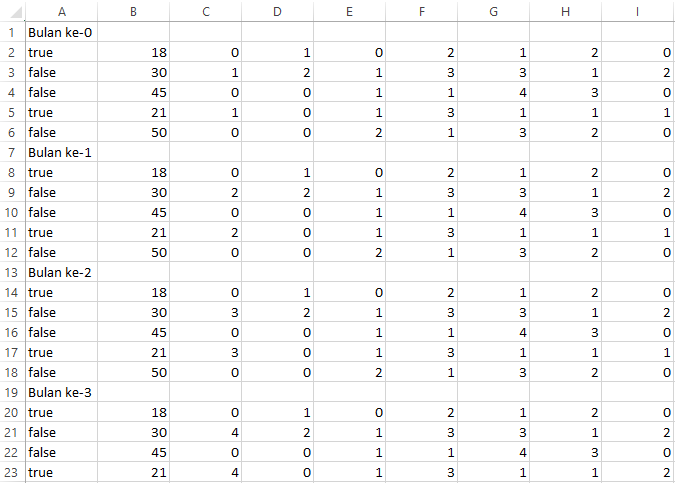
\includegraphics[width=14cm, height=10cm]{hasilExcel1} 
		\caption[Hasil keluaran perubahan individu wirausaha pada \textit{file} CSV]{Hasil keluaran perubahan individu wirausaha pada \textit{file} CSV}
	\label{fig:hasilExcel1} 
\end{figure}

		\begin{figure} [H]
	\centering  
	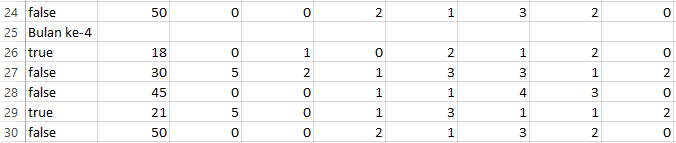
\includegraphics[width=14cm, height=4cm]{hasilExcel2} 
		\caption[Hasil keluaran perubahan individu wirausaha pada \textit{file} CSV]{Lanjutan hasil keluaran perubahan individu wirausaha pada \textit{file} CSV}
	\label{fig:hasilExcel2} 
\end{figure}
	\item Tampilan Hasil
	
	Pada tampilan ini akan ditampilkan hasil dari simulasi berupa tabel yang isi setiap kolomnya adalah iterasi (bulan), jumlah wirausaha yang berada pada level \textit{potential}, jumlah wirausaha yang berada pada level \textit{nascent}, jumlah wirausaha yang berada pada level \textit{new\_bm}, jumlah wirausaha yang berada pada level \textit{est\_bm} dan jumlah wirausaha yang berada pada level \textit{retired}. (Gambar \ref{fig:tampilanHasil})
	
	\begin{figure} [H]
	\centering  
	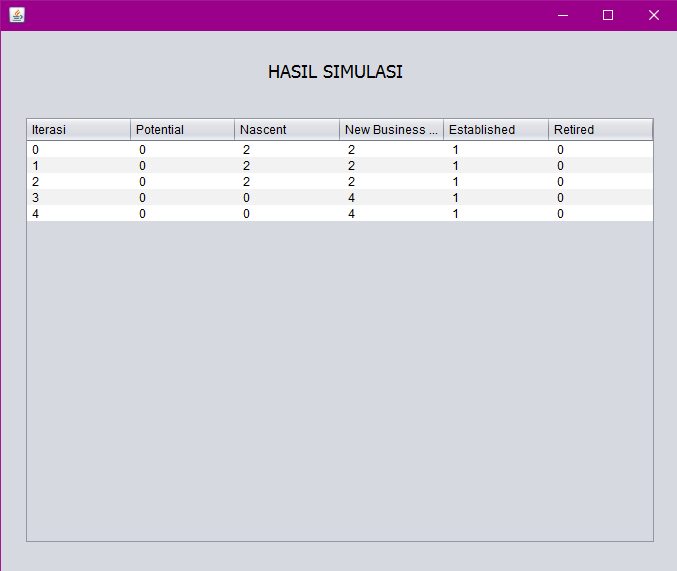
\includegraphics[width=12cm, height=10cm]{hasil2} 
		\caption[Gambar Tampilan Hasil]{Gambar Tampilan Hasil}
	\label{fig:tampilanHasil} 
\end{figure}

\end{enumerate}

\section{Pengujian}
\subsection{Pengujian Fungsional}
Pengujian fungsional dilakukan untuk mengetahui kesesuaian reaksi perangkat lunak dengan reaksi yang diharapkan berdasarkan aksi \textit{user} terhadap perangkat lunak. Pengujian ini ditujukan pada 1 pengguna yaitu \textit{user}.\\
Terdapat 8 tes kasus yang diujikan. Detail dan hasilnya dapat dilihat pada tabel \ref{tabelFungsional}

\begin{table}[H]
\centering
\caption{Tabel Pengujian Fungsional \textit{User}}
\begin{tabular}{|c|p{6cm}|p{4cm}|p{2cm}|}
\hline
No & Aksi Pengguna & Reaksi yang diharapkan & Reaksi Perangkat Lunak\\
\hline
1 & \textit{User} menjalankan simulator / aplikasi & Tampilan Bobot Ketetanggaan akan ditampilkan & Sesuai\\
\hline
2 & \textit{User} melanjutkan pengisian dengan memilih \textit{button} "NEXT" & Tampilan Kondisi Ketetanggaan akan ditampilkan & Sesuai\\
\hline
3 & \textit{User} melanjutkan pengisian dengan memilih \textit{button} "NEXT" & Tampilan Kondisi Eksternal akan ditampilkan & Sesuai\\
\hline
4 & \textit{User} melanjutkan pengisian dengan memilih \textit{button} "NEXT" & Tampilan Data Wirausaha akan ditampilkan & Sesuai\\
\hline
5 & \textit{User} memasukkan data wirausaha dengan memilih \textit{button} "OPEN FILE" & Muncul \textit{pop up windows} yang menyediakan beberapa \textit{file}, salah satu \textit{file} akan dipilih oleh \textit{user} & Sesuai\\
\hline
6 & Setelah \textit{User} memilih \textit{file} dan memilih \textit{button} "OPEN" & Data wirausaha akan ditampilkan di tabel & Sesuai\\
\hline
7 & \textit{User} melanjutkan proses simulasi dengan memilih \textit{button} "NEXT" & Tampilan Simulasi akan ditampilkan & Sesuai\\
\hline
8 & \textit{User} selesai mengisi \textit{text field} dan memilih \textit{button} "SIMULATE" & Hasil simulasi akan ditampilkan di tabel dan pada \textit{file} CSV & Sesuai\\
\hline 

\end{tabular}
\label{tabelFungsional}
\end{table} 

\subsection{Pengujian Pembacaan Parameter}
Pengujian ini dilakukan agar tidak terjadi kesalahan \textit{input} dari \textit{user} yang mengakibatkan hasil simulasi tidak sesuai dengan yang diharapkan.
\begin{enumerate}
	\item Pengisian \textit{Text Field} pada saat mengisi bobot ketetanggaan
	\begin{itemize}
		\item Jika \textit{user} sudah mengisi \textit{check box} tetapi tidak mengisi \textit{text field}, akan terdapat pesan kesalahan "You cannot move to the other page because you must fill text field first!". (Gambar \ref{pesanError1})
		
	\begin{figure} [H]
	\centering  
	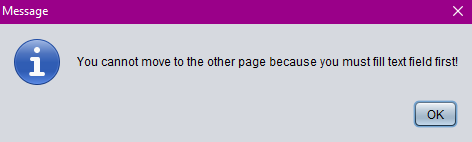
\includegraphics[width=12cm, height=4cm]{pesanError2} 
		\caption[Tampilan Pesan Error pada saat \textit{text field} tidak terisi]{Tampilan Pesan Error pada saat \textit{text field} tidak terisi}
	\label{pesanError1} 
\end{figure}
		
		\item Jika \textit{user} sudah mengisi \textit{text field} tetapi totalnya tidak 100\%, akan terdapat pesan kesalahan "The sum of text fields must 100\%!". (Gambar \ref{pesanError2})
		
	\begin{figure} [H]
	\centering  
	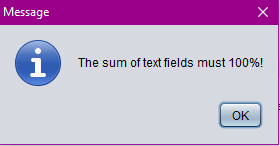
\includegraphics[width=8cm, height=4cm]{pesanError1} 
		\caption[Tampilan Pesan Error pada saat isi dari \textit{text field} tidak berjumlah 100\%]{Tampilan Pesan Error pada saat isi dari \textit{text field} tidak berjumlah 100\%}
	\label{pesanError2} 
\end{figure}

	\end{itemize}
	
	\item Pengisian \textit{Radio Button} pada saat mengisi relasi ketetanggaan\\
	Jika \textit{user} tidak mengisi radio button, akan ada pesan kesalahan yaitu "You cannot move to the other page because you must fill radio button first!". (Gambar \ref{pesanError3})
	
		\begin{figure} [H]
	\centering  
	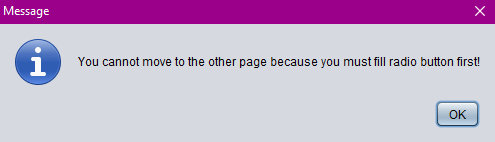
\includegraphics[width=11cm, height=4cm]{pesanError3} 
		\caption[Tampilan Pesan Error pada saat \textit{radio button} tidak terisi]{Tampilan Pesan Error pada saat \textit{radio button} tidak terisi}
	\label{pesanError3} 
\end{figure}

\item Pengisian \textit{Text Field} pada saat mengisi bobot faktor eksternal
	\begin{itemize}
		
		\item Jika \textit{user} tidak mengisi seluruh \textit{text field}, akan terdapat pesan kesalahan " You must fill the textfield!". (Gambar \ref{pesanError4})
		
	\begin{figure} [H]
	\centering  
	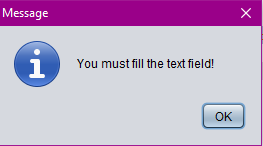
\includegraphics[width=8cm, height=4cm]{pesanError4} 
		\caption[Tampilan Pesan Error pada saat \textit{text field} tidak terisi seluruhnya]{Tampilan Pesan Error pada saat \textit{text field} tidak terisi seluruhnya}
	\label{pesanError4} 
\end{figure}
		
		\item Jika \textit{user} tidak mengisi \textit{text field}, akan terdapat pesan kesalahan "You cannot move to the other page because you must fill text field first!". (Gambar \ref{pesanError1})
		
	\begin{figure} [H]
	\centering  
	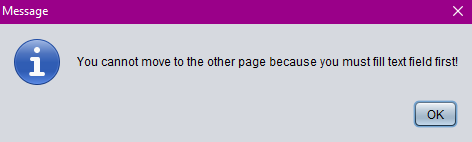
\includegraphics[width=12cm, height=4cm]{pesanError2} 
		\caption[Tampilan Pesan Error pada saat \textit{text field} tidak terisi]{Tampilan Pesan Error pada saat \textit{text field} tidak terisi}
	\label{pesanError1} 
	\end{figure}
	
	\item Jika \textit{user} sudah mengisi \textit{text field} tetapi totalnya tidak 100\%, akan terdapat pesan kesalahan "The sum of text fields must 100\%!". (Gambar \ref{pesanError2})
		
	\begin{figure} [H]
	\centering  
	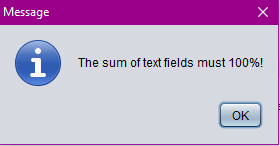
\includegraphics[width=8cm, height=4cm]{pesanError1} 
		\caption[Tampilan Pesan Error pada saat isi dari \textit{text field} tidak berjumlah 100\%]{Tampilan Pesan Error pada saat isi dari \textit{text field} tidak berjumlah 100\%}
	\label{pesanError2} 
\end{figure}
	\end{itemize}
	
	\item Pengisian nilai a,b dan c\\
	Jika \textit{user} mengisi nilai a,b dan c jumlahnya tidak 1, akan ada pesan kesalahan yaitu "The sum of a,b and c's value must 1!". (Gambar \ref{pesanError5})
	
	\begin{figure} [H]
	\centering  
	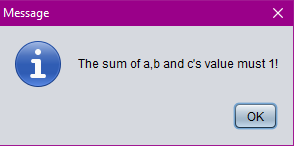
\includegraphics[width=8cm, height=4cm]{pesanError5} 
		\caption[Tampilan Pesan Error pada saat nilai a,b dan c tidak berjumlah 1]{Tampilan Pesan Error pada saat nilai a,b dan c tidak berjumlah 1}
	\label{pesanError5} 
\end{figure}
	
\end{enumerate}

\subsection{Pengujian Pembacaan File}
Pengujian ini bertujuan untuk membuktikan kebenaran antara \textit{file} masukan yang \textit{user} berikan dengan akan ditampilkan pada tabel.\\
Berikut contoh \textit{file} data wirausaha yang diberikan \textit{user} (Gambar \ref{formatFile})

	\begin{figure} [H]
	\centering  
	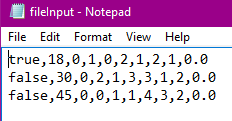
\includegraphics[width=8cm, height=4cm]{formatFile} 
		\caption[Contoh format \textit{file} data wirausaha]{Contoh format \textit{file} data wirausaha}
	\label{formatFile} 
\end{figure}

Berikut hasil yang ditampilkan pada tabel : (Gambar \ref{tampilanData})

	\begin{figure} [H]
	\centering  
	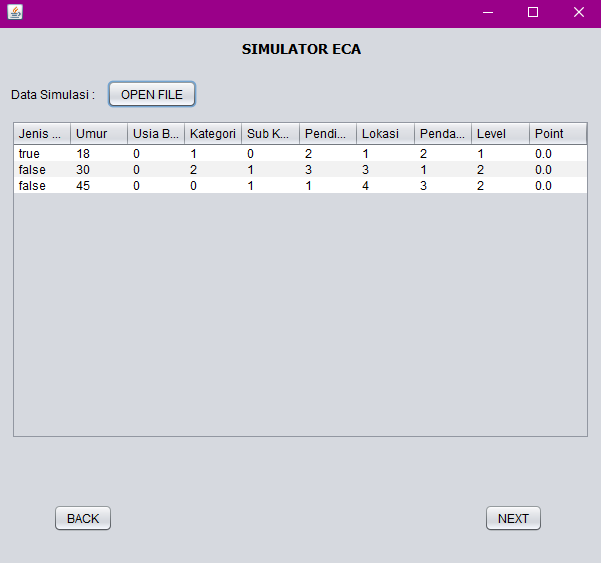
\includegraphics[width=12cm, height=12cm]{tampilanData} 
		\caption[Contoh format \textit{file} data wirausaha]{Contoh format \textit{file} data wirausaha}
	\label{tampilanData} 
\end{figure}

Pada pengujian pembacaan \textit{file} data wirausaha jika \textit{user} tidak memasukkan \textit{file} data wirausaha, akan ada pesan kesalahan berupa "You must choose the file first!". (Gambar \ref{pesanError6})

	\begin{figure} [H]
	\centering  
	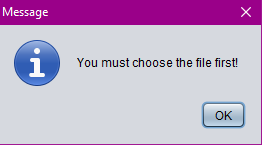
\includegraphics[width=8cm, height=4cm]{pesanError6} 
		\caption[Tampilan pesan kesalahan apabila \textit{file} data wirausaha belum dipilih]{Tampilan pesan kesalahan apabila \textit{file} data wirausaha belum dipilih}
	\label{pesanError6} 
\end{figure}

 
\subsection{Pengujian Hasil dari Simulasi}

Pengujian ini bertujuan untuk menguji hasil perhitungan CIDx dari program sama dengan hasil perhitungan secara manual.\\
Contoh perhitungan menggunakan hasil perhitungan dari bab \ref{chap:analisis} pada subbab \ref{analisismodelCA}.
\begin{itemize}
\item Hasil Perhitungan CIDx Program\\
	Berikut hasil perhitungan \textit{Continuity Index} untuk masing-masing wirausahawan:
	\begin{itemize}
		\item Iterasi pada bulan pertama\\
		Dapat dilihat pada gambar \ref{hasilIterasi0} hasil dari masing-masing wirausahawan mulai dari wirausahawan 1,2 dan 3 pada iterasi pertama.
	\begin{figure} [H]
	\centering  
	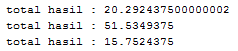
\includegraphics[width=6cm, height=3cm]{hasilIterasi0} 
		\caption[Hasil Iterasi bulan pertama]{Hasil iterasi bulan pertama}
	\label{hasilIterasi0} 
\end{figure}
	 20.2924
		\item Iterasi pada bulan kedua\\
		Dapat dilihat pada gambar \ref{hasilIterasi1} hasil dari masing-masing wirausahawan mulai dari wirausahawan 1,2 dan 3 pada iterasi kedua.
	\begin{figure} [H]
	\centering  
	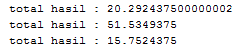
\includegraphics[width=6cm, height=3cm]{hasilIterasi1} 
		\caption[Hasil Iterasi bulan kedua]{Hasil iterasi bulan kedua}
	\label{hasilIterasi1} 
\end{figure}
		\item Iterasi pada bulan ketiga\\
		Dapat dilihat pada gambar \ref{hasilIterasi2} hasil dari masing-masing wirausahawan mulai dari wirausahawan 1,2 dan 3 pada iterasi ketiga.
		
	\begin{figure} [H]
	\centering  
	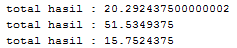
\includegraphics[width=6cm, height=3cm]{hasilIterasi2} 
		\caption[Hasil Iterasi bulan ketiga]{Hasil iterasi bulan ketiga}
	\label{hasilIterasi2} 
\end{figure}
		\item Iterasi pada bulan keempat\\
		Dapat dilihat pada gambar \ref{hasilIterasi3} hasil dari masing-masing wirausahawan mulai dari wirausahawan 1,2 dan 3 pada iterasi keempat
	\begin{figure} [H]
	\centering  
	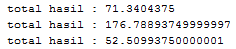
\includegraphics[width=6cm, height=3cm]{hasilIterasi3} 
		\caption[Hasil Iterasi bulan keempat]{Hasil iterasi bulan keempat}
	\label{hasilIterasi3} 
\end{figure}

		\item Iterasi pada bulan kelima\\
		Dapat dilihat pada gambar \ref{hasilIterasi4} hasil dari masing-masing wirausahawan mulai dari wirausahawan 1,2 dan 3 pada iterasi kelima.
	\begin{figure} [H]
	\centering  
	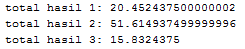
\includegraphics[width=6cm, height=3cm]{hasilIterasi4} 
		\caption[Hasil Iterasi bulan kelima]{Hasil iterasi bulan kelima}
	\label{hasilIterasi4} 
\end{figure}
		
	\end{itemize}

\item Hasil Perhitungan CIDx Manual\\
Berikut hasil dari perhitungan CIDx manual :
	\begin{table}[H]
	\centering
	\begin{tabular}{|c|c|c|c|}
	\hline
	& Entrepreneur 1 & Entrepreneur 2 & Entrepreneur 3\\
	\hline
	Bulan pertama & 20.09243 & 51.3749 & 15.4374\\
	\hline
	Bulan kedua & 20.09243 & 51.3749 & 15.4374\\
	\hline
	Bulan ketiga & 20.09243 & 51.3749 & 15.4374\\
	\hline
	Bulan keempat & 20.2124 & 51.4349 & 15.4974\\
	\hline
	Bulan kelima & 20.2124 & 51.4349 & 15.4974\\
	\hline
	\end{tabular}
	\end{table}
\end{itemize}

\section{Contoh Simulasi}
Diberikan contoh simulasi untuk penelitian ini yaitu sebagai berikut :\\
Sebuah populasi yang terdiri dari 60 wirausaha. Pada simulasi ini digunakan tiga buah kriteria ketetanggaan, yaitu: level wirausaha, bidang usaha dan lokasi usaha. Masing-masing bobotnya yaitu 30\%, 40\% dan 30\%. Contoh simulasi ini mengacu pada \cite{GEM2013} untuk perhitungan kondisi publik. Tujuan dari contoh simulasi ini adalah untuk menunjukkan pengaruh dari komposisi a,b,c dan \textit{threshold}. Masing-masing simulasi sebanyak enam kali dengan parameter yang diberikan pada tabel \ref{tabelParameter}. Masing-masing simulasi terdiri atas 36 iterasi yang merepresentasikan 36 bulan atau 3 tahun. Pada penelitian ini dimisalkan 1 iterasi adalah 1 bulan.
\begin{table}[H]
\centering
\caption{Tabel Parameter Settings}
\begin{tabular}{|c|c|c|c|c|}
\hline
Simulasi & a & b & c & \textit{threshold}\\
\hline
1 & 0.7 & 0.2 & 0.1 & 20\\
\hline 
2 & 0.6 & 0.3 & 0.1 & 20\\
\hline
3 & 0.5 & 0.4 & 0.1 & 20\\
\hline
4 & 0.5 & 0.3 & 0.2 & 20\\
\hline
5 & 0.5 & 0.3 & 0.2 & 15\\
\hline
6 & 0.5 & 0.3 & 0.2 & 10\\
\hline
7 & 0.6 & 0.2 & 0.2 & 20\\
\hline
8 & 0.5 & 0.2 & 0.3 & 20\\
\hline
9 & 0.4 & 0.2 & 0.4 & 20\\
\hline 
\end{tabular}
\label{tabelParameter}
\end{table}
Hasil simulasi akan diberikan pada gambar \ref{grafik1}, \ref{grafik2}, \ref{grafik3}, \ref{grafik4}, \ref{grafik5}, \ref{grafik6}, \ref{grafik7}, \ref{grafik8} dan \ref{grafik9}, dimana sumbu x menyatakan lamanya iterasi berjalan (bulan) dan sumbu y menyatakan jumlah wirausahawan.
	\begin{figure} [H]
	\centering  
	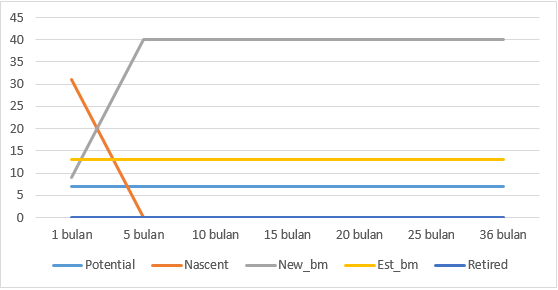
\includegraphics[width=10cm, height=6cm]{grafik1} 
		\caption[Hasil dari simulasi]{Hasil dari simulasi 1}
	\label{grafik1} 
\end{figure}

	\begin{figure} [H]
	\centering  
	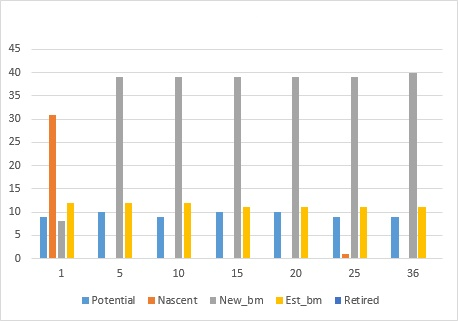
\includegraphics[width=10cm, height=6cm]{grafik2} 
		\caption[Hasil dari simulasi]{Hasil dari simulasi 2}
	\label{grafik2} 
\end{figure}

	\begin{figure} [H]
	\centering  
	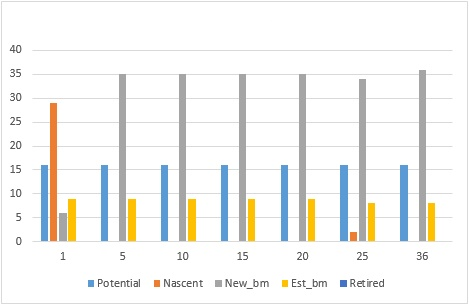
\includegraphics[width=10cm, height=6cm]{grafik3} 
		\caption[Hasil dari simulasi]{Hasil dari simulasi 3}
	\label{grafik3} 
\end{figure}

Dapat dilihat pada gambar \ref{grafik1}, \ref{grafik2} dan \ref{grafik3} menunjukkan bahwa semakin besar pengaruh tetangga maka pertumbuhan wirausaha semakin melambat hal ini dapat dibuktikan pada jumlah wirausaha \textit{est\_bm} yang menurun dari tahun pertama sampai tahun ketiga.

	\begin{figure} [H]
	\centering  
	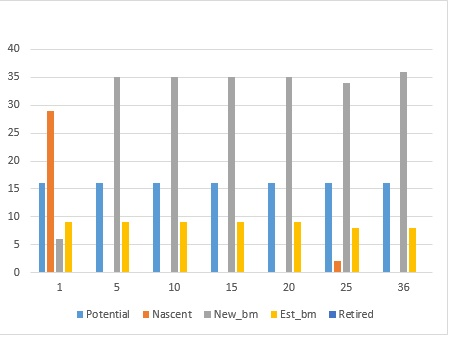
\includegraphics[width=10cm, height=6cm]{grafik4} 
		\caption[Hasil dari simulasi]{Hasil dari simulasi 4}
	\label{grafik4} 
\end{figure}

	\begin{figure} [H]
	\centering  
	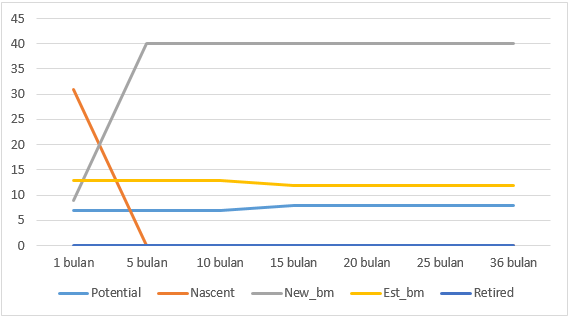
\includegraphics[width=10cm, height=6cm]{grafik5} 
		\caption[Hasil dari simulasi]{Hasil dari simulasi 5}
	\label{grafik5} 
\end{figure}

	\begin{figure} [H]
	\centering  
	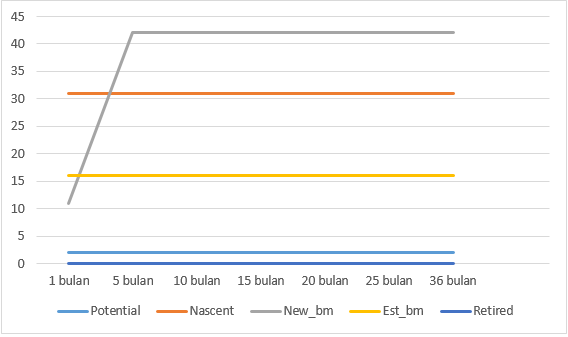
\includegraphics[width=10cm, height=6cm]{grafik6} 
		\caption[Hasil dari simulasi]{Hasil dari simulasi 6}
	\label{grafik6} 
\end{figure}

Dapat dilihat pada gambar \ref{grafik4}, \ref{grafik5} dan \ref{grafik6} menunjukkan bahwa wirausaha \textit{new\_bm} dan \textit{est\_bm} berbanding terbalik dengan nilai \textit{threshold}.

	\begin{figure} [H]
	\centering  
	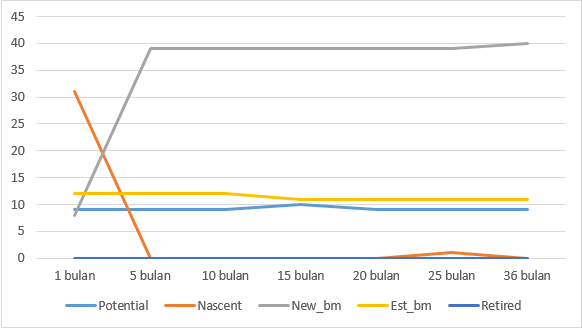
\includegraphics[width=10cm, height=6cm]{grafik7} 
		\caption[Hasil dari simulasi]{Hasil dari simulasi 7}
	\label{grafik7} 
\end{figure}

	\begin{figure} [H]
	\centering  
	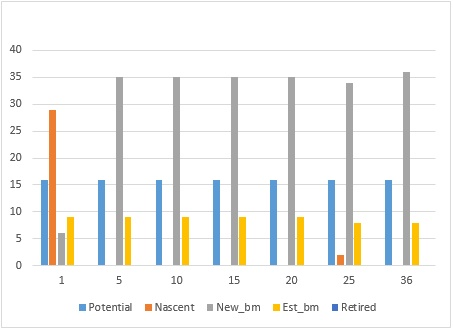
\includegraphics[width=10cm, height=6cm]{grafik8} 
		\caption[Hasil dari simulasi]{Hasil dari simulasi 8}
	\label{grafik8} 
\end{figure}

	\begin{figure} [H]
	\centering  
	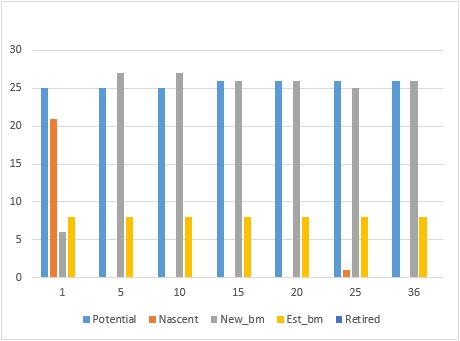
\includegraphics[width=10cm, height=6cm]{grafik9} 
		\caption[Hasil dari simulasi]{Hasil dari simulasi 9}
	\label{grafik9} 
\end{figure}

Dapat dilihat pada gambar \ref{grafik7}, \ref{grafik8} dan \ref{grafik9} menunjukkan bahwa semakin besar faktor publik maka pertumbuhan wirausaha semakin melambat hal ini dapat dilihat dari menurunnya jumlah wirausaha \textit{new\_bm}, wirausaha \textit{nascent} dan wirausaha \textit{est\_bm}.
%wirausaha \textit{potential} yang menjadi wirausaha \textit{nascent} menurun, hal ini dibuktikan dengan menurunnya jumlah wirausaha \textit{nascent} dan meningkatnya jumlah wirausaha \textit{potential}. Tetapi semakin banyak jumlah wirausaha \textit{nascent} yang menjadi wirausaha \textit{new_bm}, hal ini dibuktikan dengan meningkatnya jumlah wirausaha \textit{new_bm} dari tahun 1 sampai tahun ketiga. Wirausaha \textit{est_bm} jumlahnya juga menurun.
